As mentioned before, the \gls{rgb} state is the default representation of the
Q*bert Atari environment. The \gls{rgb} state is a three-dimensional tensor
where each dimension represents the red, green, and blue channels of the
environment, and has a size of 210x160x3, which is a large representation of
the environment. The \gls{rgb} state and its scaled down version are shown in
\cref{fig:rgb-state}.

\begin{figure}[H]
    \centering
    \begin{subfigure}{0.45\textwidth}
        \centering
        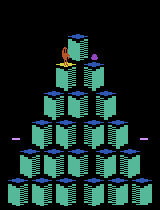
\includegraphics[width=\textwidth]{img/rgb-full-purple.png}
        \caption{Full state representation.}
        \label{fig:rgb-full}
    \end{subfigure}
    \begin{subfigure}{0.45\textwidth}
        \centering
        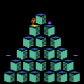
\includegraphics[width=\textwidth]{img/rgb-84x84-purple.png}
        \caption{84x84 state representation.}
        \label{fig:rgb-84x84}
    \end{subfigure}
    \caption{RGB state representation.}
    \label{fig:rgb-state}
\end{figure}

As we see in \cref{fig:rgb-full}, the scaled down version of the \gls{rgb}
state, as shown in \cref{fig:rgb-84x84}, keeps the main features of the
environment, such as the platforms, the enemies, and the player.